%*----------- SLIDE -------------------------------------------------------------
\begin{frame}[c]{}
    \begin{center}
        \Wider{%
        \begin{shaded}
        \begin{center}
            \vspace*{0.8cm}
            \resizebox{!}{1cm}{%
               % \color{bg} O objetivo é ter um objetivo.
                \begin{tabular}{ccc}
                    \textbf{Projetos}   
                  \end{tabular}
            }%
        \end{center}
        \end{shaded}
        }%
    \end{center}
%*----------- notes
    \note[item]{Notes can help you to remember important information. Turn on the notes option.}
\end{frame}
%-
%*----------- SLIDE -------------------------------------------------------------
\begin{frame}[t]{FlatFish@ROS}
    Atualizar o framework utilizado no protótipo do FlatFish, migrando para o ROS.
    
    \begin{center}
    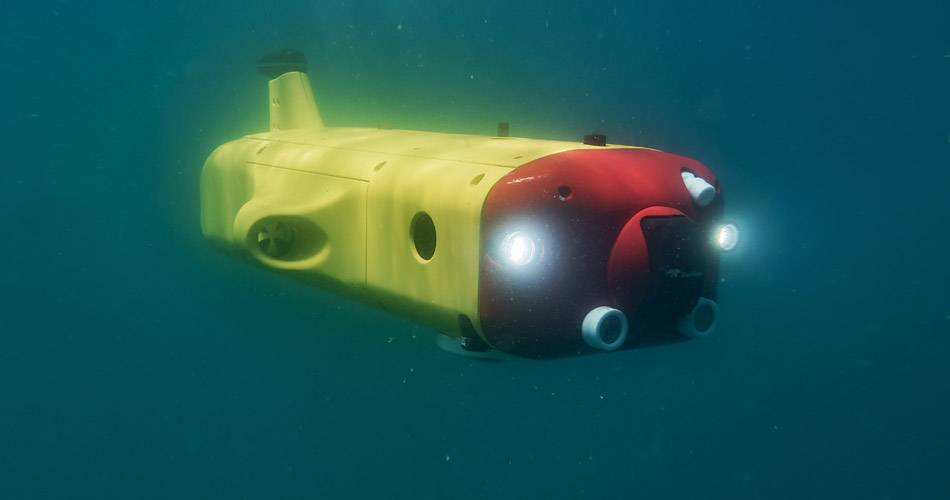
\includegraphics[width=0.5\textwidth]{flatfish.jpg}
    \end{center}
    
    
            
\end{frame}
%*----------- SLIDE -------------------------------------------------------------
\begin{frame}[t]{FlatFish@ROS}
    \framesubtitle{Desenvolvido}
    \begin{itemize}
        \item Elaborado o cronograma do projeto
        \item Estudo ROS
        \item Conexão do computador central FlatFISH
        \item Ajustes na NUC
    \end{itemize}    
%*----------- notes
    \note[item]{Notes can help you to remember important information. Turn on the notes option.}
\end{frame}
%-
%*----------- SLIDE -------------------------------------------------------------
\begin{frame}[t]{FlatFish@ROS}
    \framesubtitle{Próximos passos}
    \begin{itemize}
        \item Listar as funcionalidades para desenvolvimento da montagem do sistema robótico submarino
        \item Simulação no openFOAM
        \item Simulação no ROS
        \item Desenvolvimento de 4 artigos: 
        \begin{itemize}
            \item[] 2022- SOTA e Simulação OpenFOAM
            \item[] 2023- DOE OpenFOAM e ROS 
        \end{itemize}  
        
    \end{itemize}    
%*----------- notes
    \note[item]{Notes can help you to remember important information. Turn on the notes option.}
\end{frame}
%-


\begin{frame}[t]{Pirabots}
     Implmentar ações autônomas em ROVs: BlueROV e BirROV.
      
   
    \begin{columns}
        \column{.45\linewidth}
    \begin{center}

        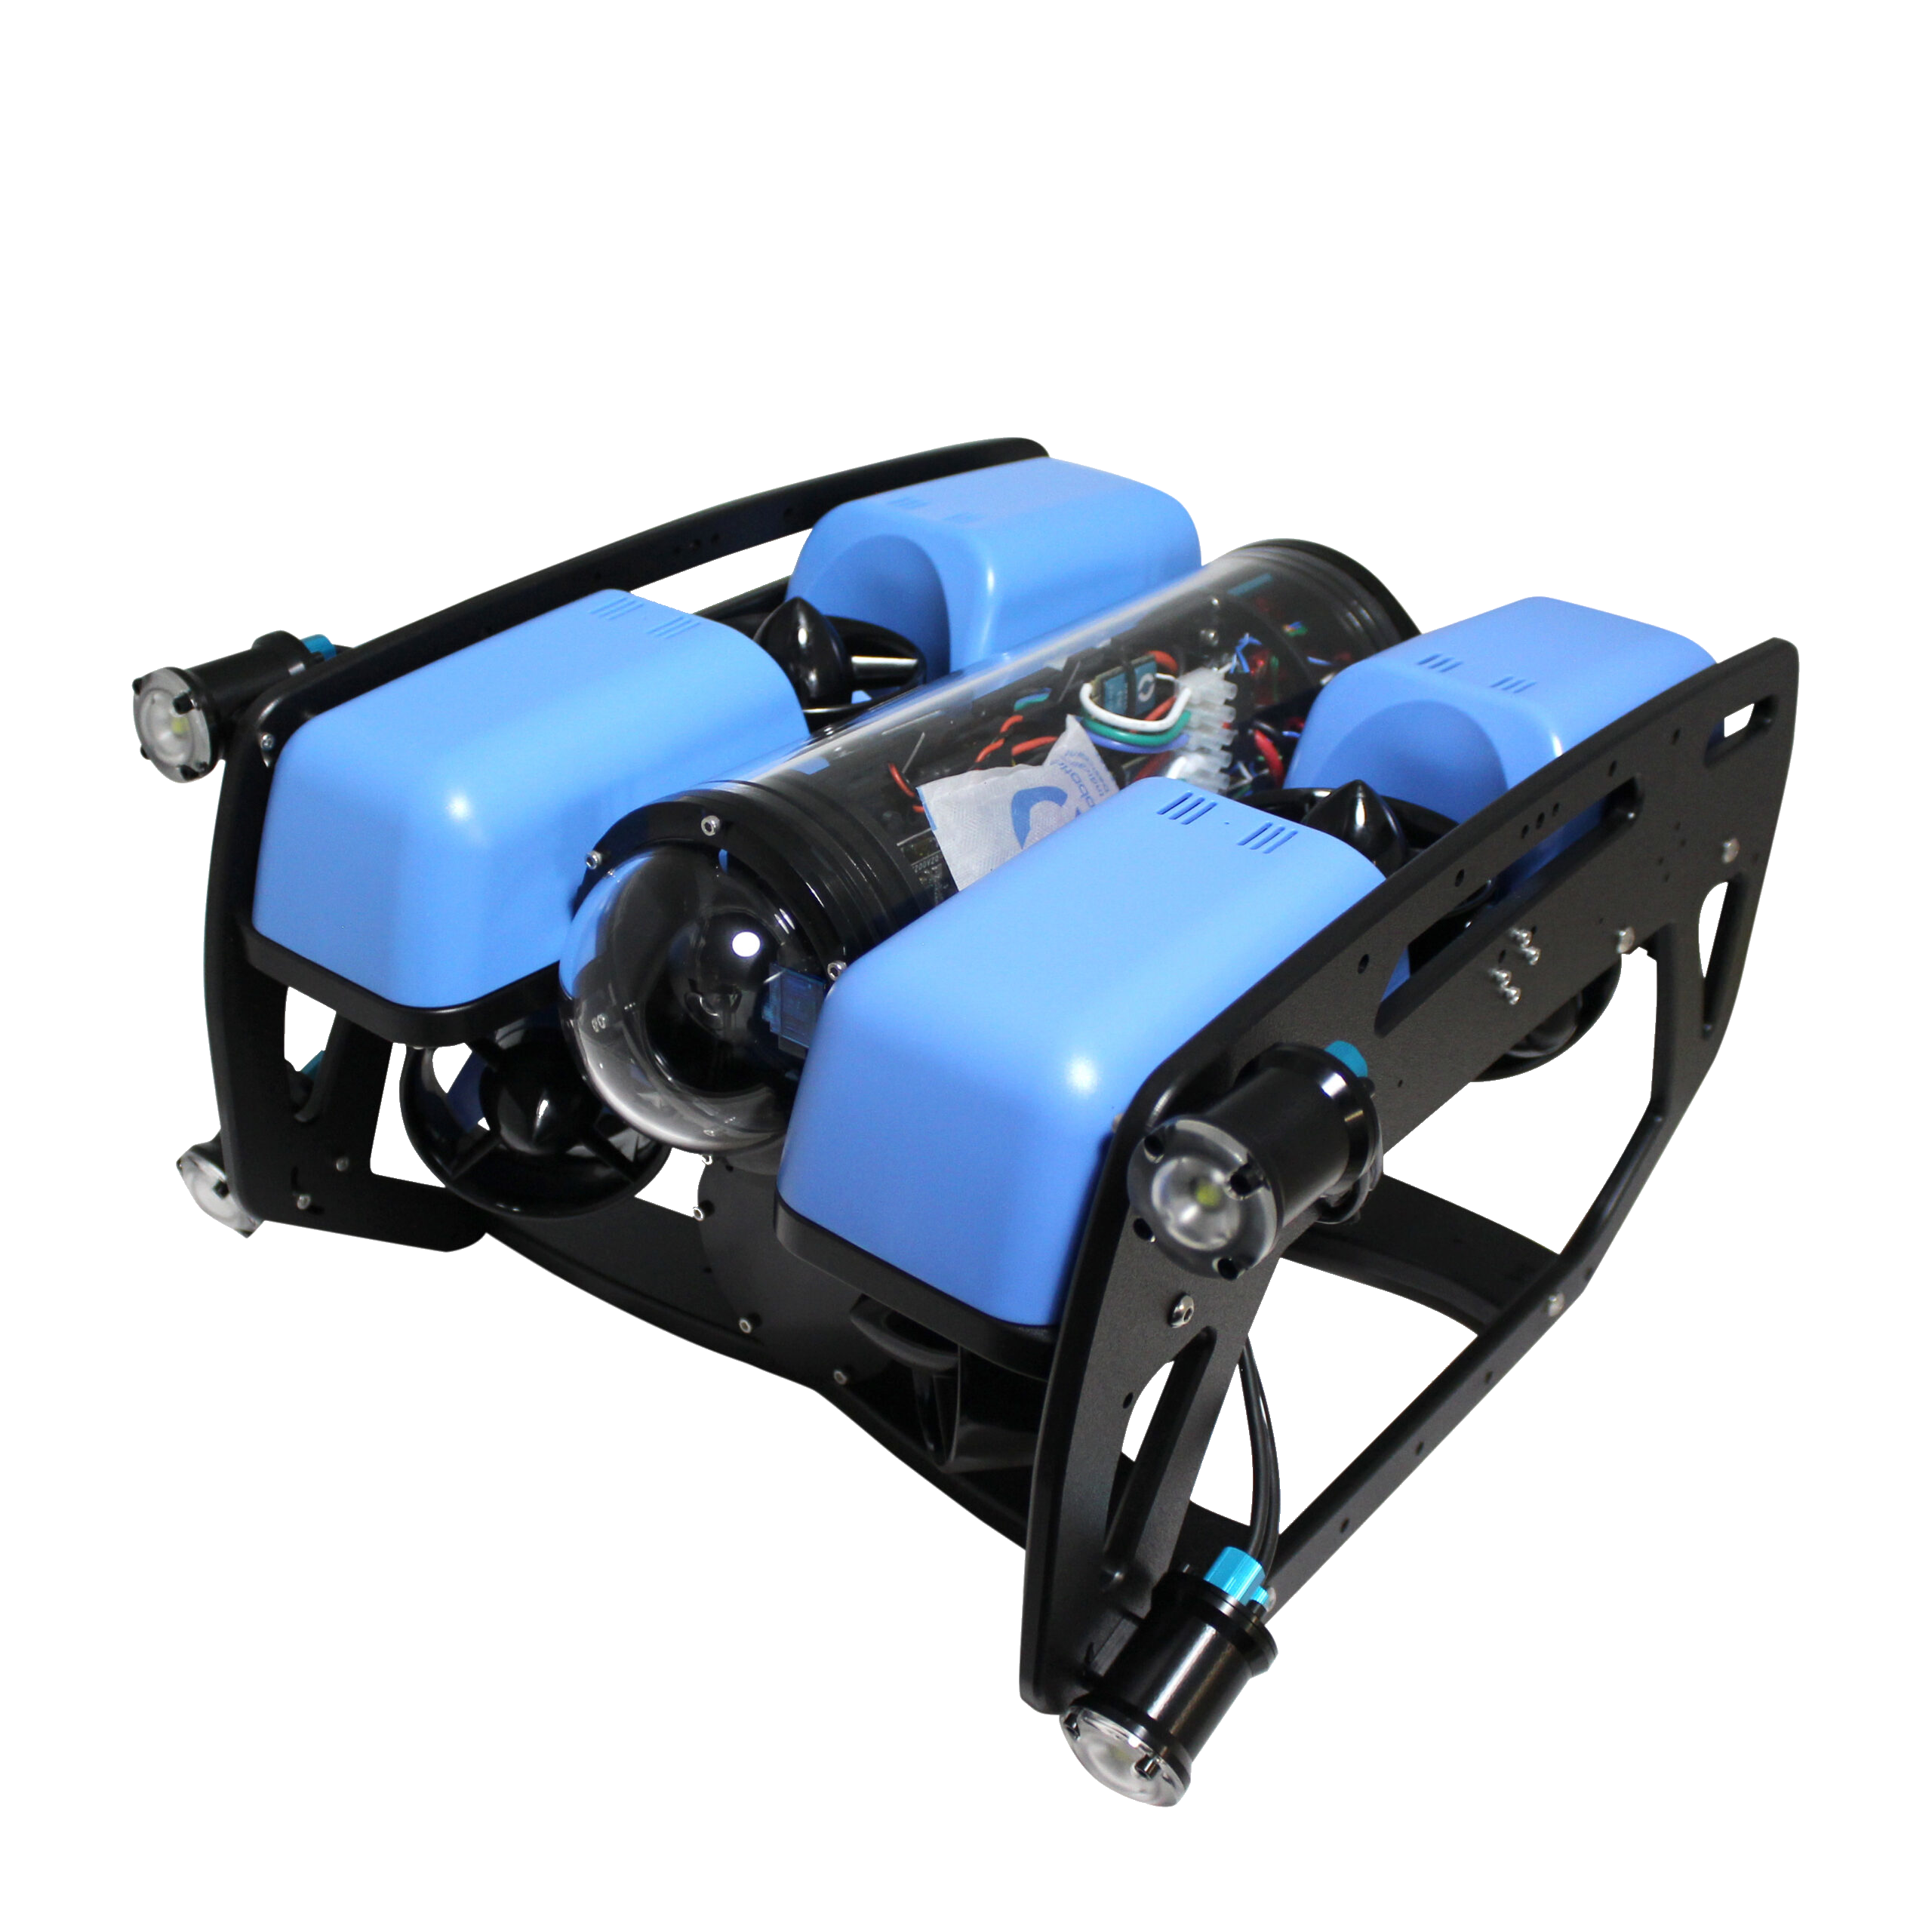
\includegraphics[width=0.8\textwidth]{bluerov.png}

    \end{center}

    \column{.45\linewidth}
    \vspace*{0.3cm}
    \begin{center}

        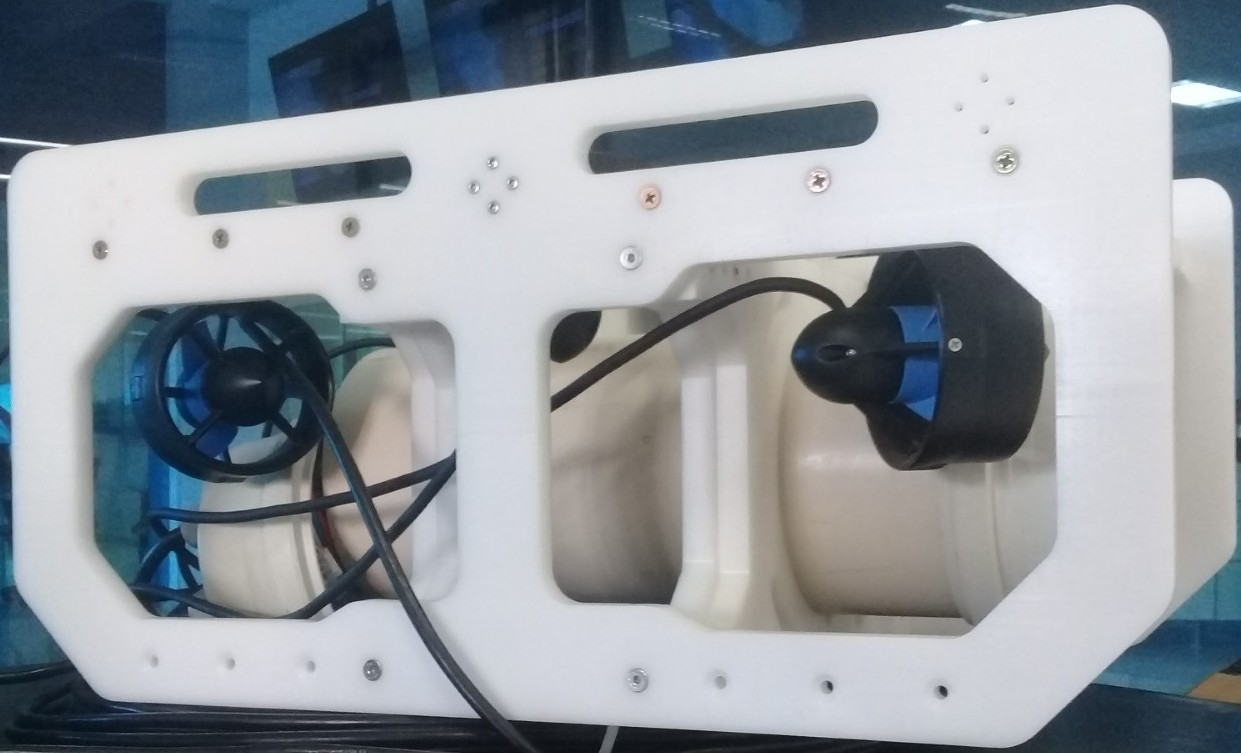
\includegraphics[width=0.8\textwidth]{bir_rov.jpg}

    \end{center}

\end{columns}

\end{frame}
%*----------- SLIDE -------------------------------------------------------------
\begin{frame}[t]{Pirabots}
    \framesubtitle{Desenvolvido}
    \begin{itemize}
        \item Elaborado o cronograma do projeto
        \item Estudo ROS
        \item Desenvlvimento do SOTA sobre ROV semi-autônomo
        \item Simulações no tanque do CIMATEC
    \end{itemize}    
%*----------- notes
    \note[item]{Notes can help you to remember important information. Turn on the notes option.}
\end{frame}
%-
%*----------- SLIDE -------------------------------------------------------------
\begin{frame}[t]{Pirabots}
    \framesubtitle{Próximos passos}
    \begin{itemize}
        \item Listar as funcionalidades para desenvolvimento da montagem do sistema robótico submarino
        \item Simulação no openFOAM
        \item Simulação no ROS
        \item Desenvolvimento de 4 artigos: 
        \begin{itemize}
            \item[] 2022- SOTA e Simulação OpenFOAM
            \item[] 2023- DOE OpenFOAM e ROS 
        \end{itemize}  
        
    \end{itemize}    
%*----------- notes
    \note[item]{Notes can help you to remember important information. Turn on the notes option.}
\end{frame}
%-

%*----------- SLIDE -------------------------------------------------------------
\begin{frame}[c]{turBOT}
    Desenvolver um veículo submarino autônomo para atuar em águas rasas para fins exploratórios,
    o veículo em desenvolvimento terá capacidade de identificar algumas anomalias ou padrões construídos
    e disponibilizará para os pesquisadores, apresenta uma dimensão menor do que os veículos comerciais.
    \begin{figure}
        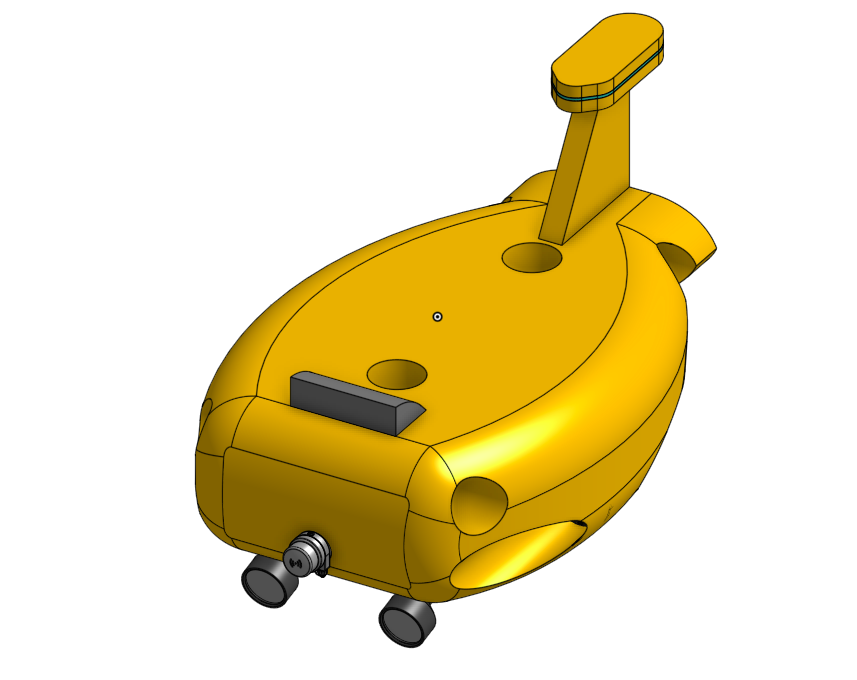
\includegraphics[width=.4\textwidth]{turbot-fish-01modi.png}
    \end{figure}
    
%*----------- notes
    \note[item]{Notes can help you to remember important information. Turn on the notes option.}
\end{frame}
%-
%*----------- SLIDE -------------------------------------------------------------
\begin{frame}[c]{turBOT }
    \framesubtitle{Metodologia}
    %\transboxin[duration=1,direction=30]
        \begin{figure}
        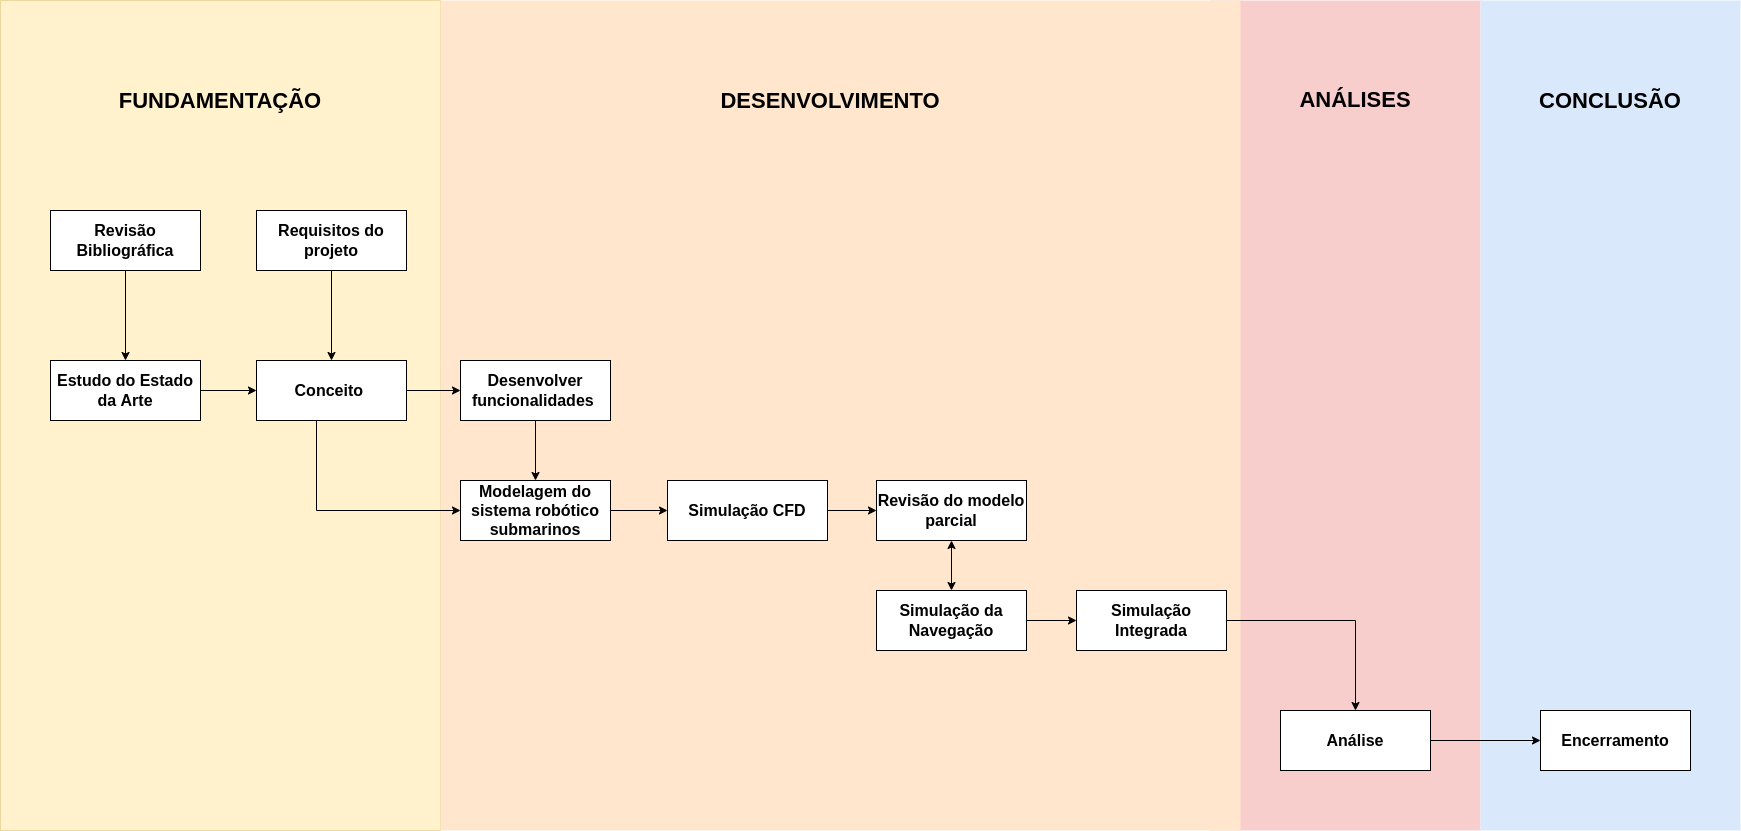
\includegraphics[width=.9\textwidth]{metodolodia-Page-2.png}
    \end{figure}
%*----------- notes
    \note[item]{Notes can help you to remember important information. Turn on the notes option.}
\end{frame}
%-
%*----------- SLIDE -------------------------------------------------------------
\begin{frame}[t]{turBOT}
    \framesubtitle{Desenvolvido}
    \begin{itemize}
        \item Elaborado o cronograma do projeto
        \item Realizado o método BiLi
        \item Estudos sobre linguagens de programação C++, Python e R
        \item Estudo ROS e openFOAM
        \item Estudo sobre CFD (Fluidodinâmica computacional)
    \end{itemize}    
%*----------- notes
    \note[item]{Notes can help you to remember important information. Turn on the notes option.}
\end{frame}
%-
%*----------- SLIDE -------------------------------------------------------------
\begin{frame}[t]{turBOT}
    \framesubtitle{Próximos passos}
    \begin{itemize}
        \item Listar as funcionalidades para desenvolvimento da montagem do sistema robótico submarino
        \item Simulação no openFOAM
        \item Simulação no ROS
        \item Desenvolvimento de 4 artigos: 
        \begin{itemize}
            \item[] 2022- SOTA e Simulação OpenFOAM
            \item[] 2023- DOE OpenFOAM e ROS 
        \end{itemize}  
        
    \end{itemize}    
%*----------- notes
    \note[item]{Notes can help you to remember important information. Turn on the notes option.}
\end{frame}
%-